\section{Results and Discussion}\label{sec:mea-system-modeling-results}
On the 31 pressure records solved by both models, the SSM+DS activity calculation is less accurate than the ideal-activity baseline.  It improves 4 records and worsens 27, with median absolute \(\log_{10}\) pressure residuals of 0.495 and 0.160, respectively.  The activity calculation converges across all 161 pressure records and 74 NMR states.  On the 66 NMR states excluded from parameter estimation, its closest speciation agreement occurs for the amine family.

\subsection{Ideal CO2 solubility baseline}
The ideal Smith--Missen-style baseline solves the five-reaction, nine-species problem with activities equal to mole fractions.  It checks the reaction and balance conventions before introducing ePC-SAFT activity coefficients.  Median absolute \(\log_{10}(\mathrm{model}/\mathrm{data})\) residuals for positive measured values are 0.055 for \MEA, 0.044 for \MEAH, 0.029 for \MEACOO, 0.227 for \HCOthree, and 0.0087 for the \ce{MEA + MEAH+} aggregate.  Molecular \COtwo and \COthree appear in the solved profiles but do not contribute to these major-species metrics.

For the 31 Jou et al.\ measurements used in the controlled comparison, the pressure baseline has a median absolute \(\log_{10}\) residual of 0.160, a signed median of \(-0.024\), and an RMSE of 0.297.  Residuals are larger at 40 and \SI{60}{\degreeCelsius} than at 80, 100, and \SI{120}{\degreeCelsius}.  These results establish the ideal reaction and balance baseline for the activity-model comparison.

\begin{center}
    \begin{minipage}{\linewidth}
    \centering
    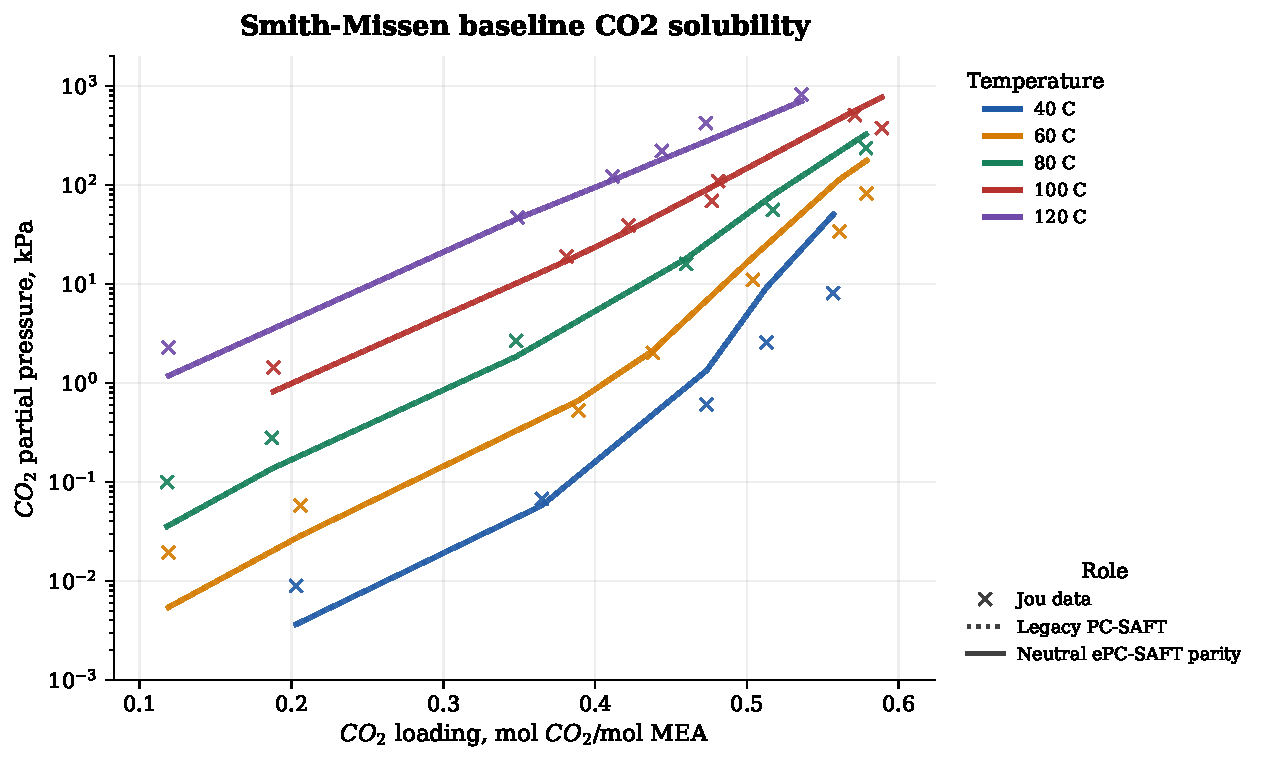
\includegraphics[width=0.84\linewidth,height=0.40\textheight,keepaspectratio]{figures/mea_ideal_pressure_vs_loading.pdf}
    \captionsetup{hypcap=false}
    \captionof{figure}{Ideal-equilibrium \COtwo-solubility pressure baseline for 30 wt\% \MEA.  Predicted pressure increases with loading at every temperature, with larger deviations at 40 and \SI{60}{\degreeCelsius} than at 80, 100, and \SI{120}{\degreeCelsius}.}
    \label{fig:ideal-pressure}
    \end{minipage}
\end{center}

\begin{center}
    \begin{minipage}{\linewidth}
    \centering
    \begin{minipage}{0.47\linewidth}
        \centering
        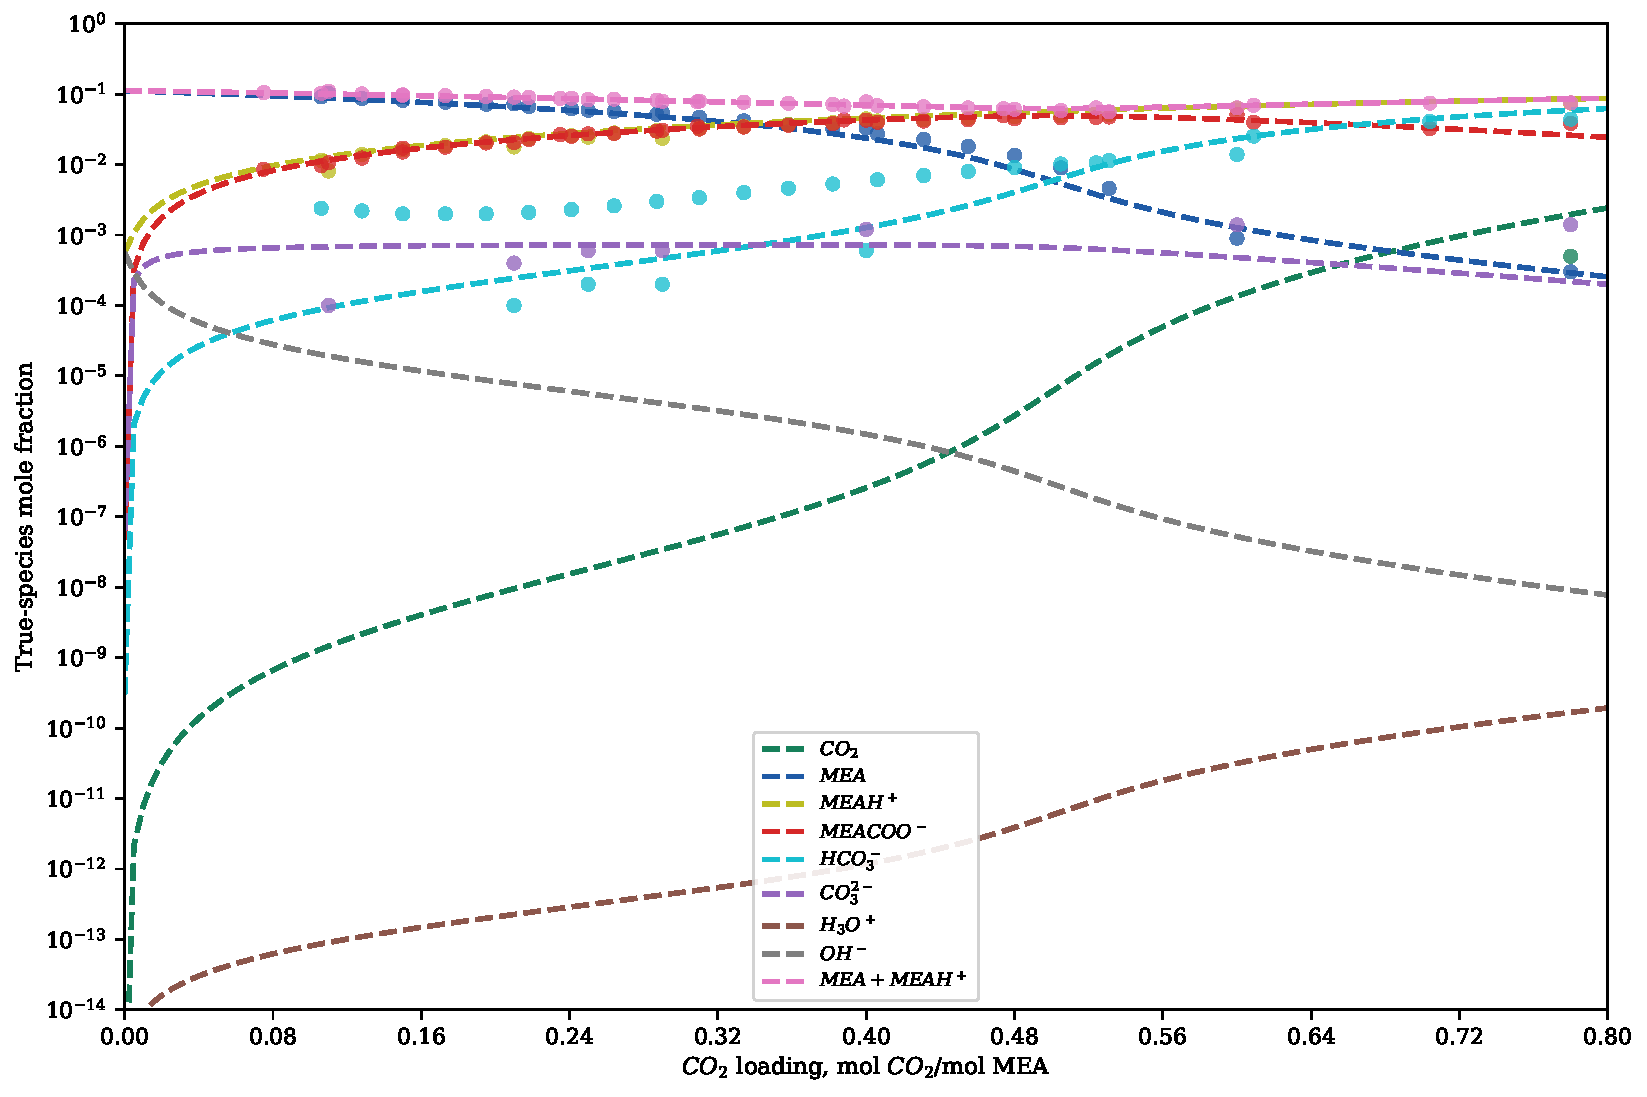
\includegraphics[width=\linewidth,height=0.30\textheight,keepaspectratio]{figures/mea_ideal_speciation_20C.pdf}
        \par\smallskip
        \small (a) \SI{20}{\degreeCelsius}
    \end{minipage}
    \hfill
    \begin{minipage}{0.47\linewidth}
        \centering
        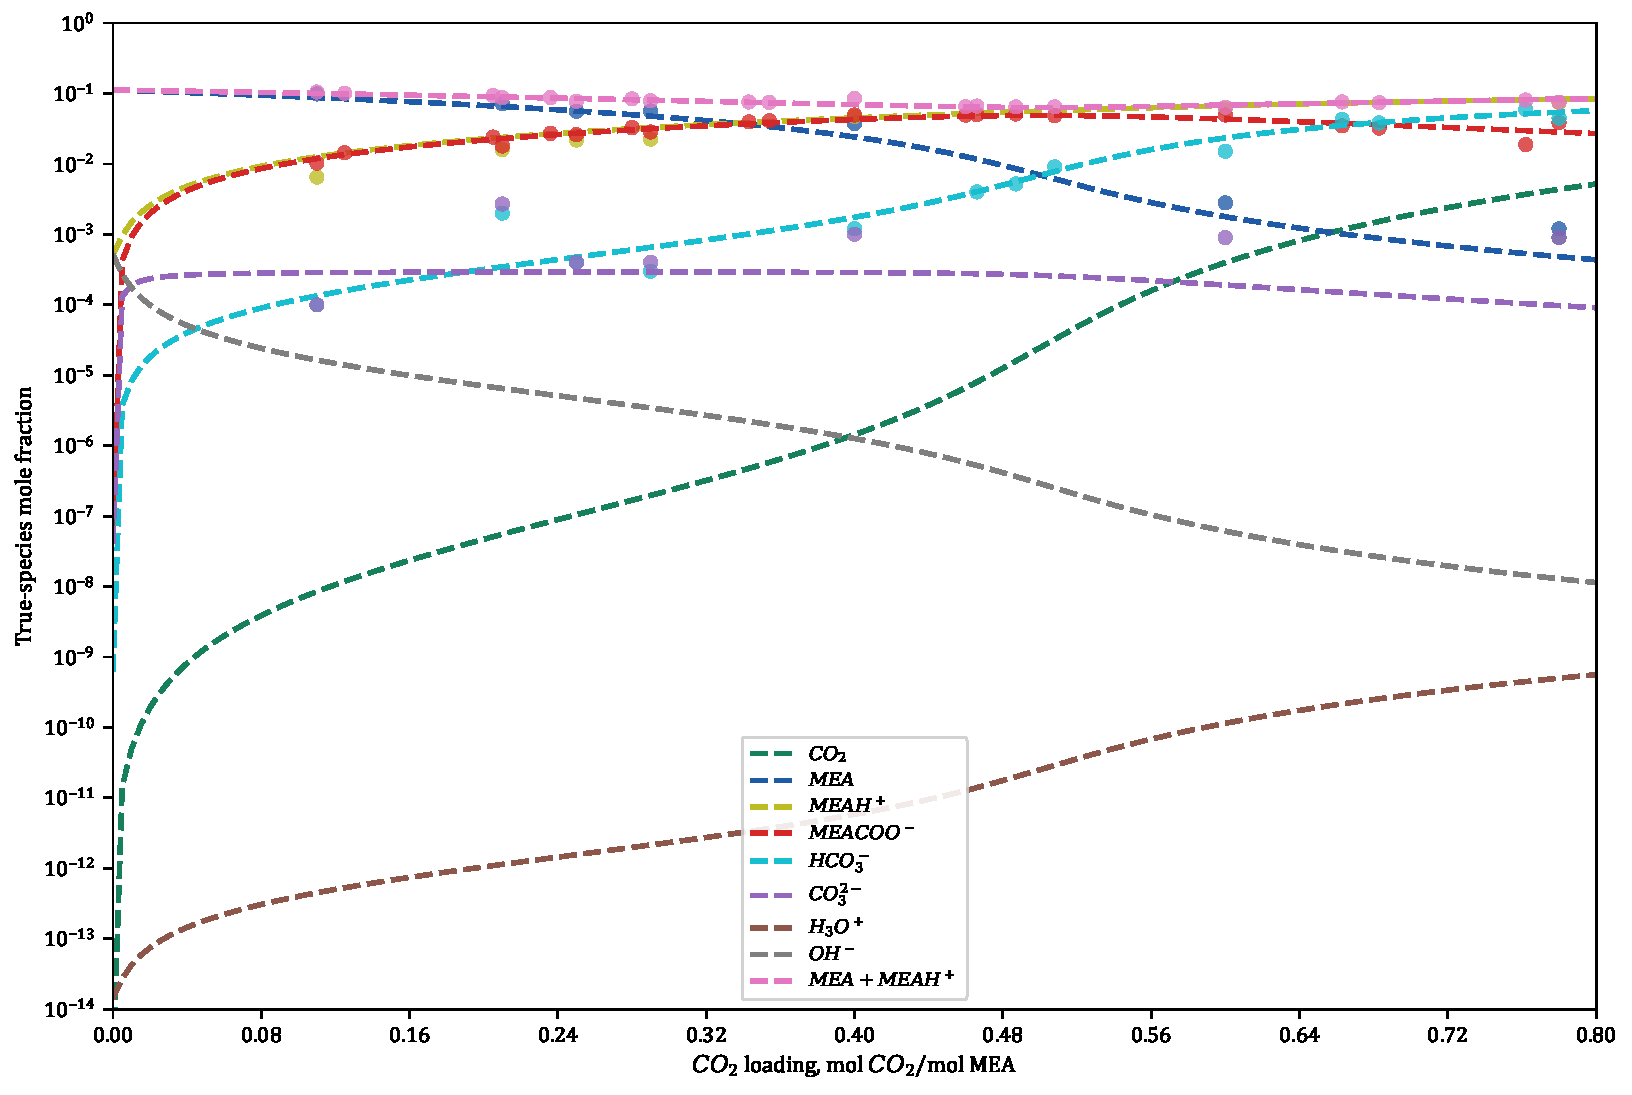
\includegraphics[width=\linewidth,height=0.30\textheight,keepaspectratio]{figures/mea_ideal_speciation_40C.pdf}
        \par\smallskip
        \small (b) \SI{40}{\degreeCelsius}
    \end{minipage}
    \captionsetup{hypcap=false}
    \captionof{figure}{Ideal-equilibrium true-species baseline for 30 wt\% \MEA.  Smooth curves show the five-reaction, nine-species equilibrium calculation; markers show literature values after declared composition-basis conversion.  Positive measured amine and bicarbonate values enter the residual comparison, while other species document the solved equilibrium state.}
    \label{fig:ideal-speciation}
    \end{minipage}
\end{center}

\subsection{Activity-based CO2 solubility model}
The activity calculation uses the nine-species basis and parameter hierarchy in \cref{sec:data-methods}.  As loading changes, it updates ionic composition, bulk permittivity, and modified-Born solvation within the activity coefficients.  The resulting liquid composition enters the \COtwo fugacity calculation, so one fixed thermodynamic state determines both pressure and speciation.

\subsection{Chemical speciation}
For the 66 NMR states excluded from parameter estimation, median absolute \(\log_{10}(\mathrm{model}/\mathrm{data})\) residuals for positive measurements are 0.065 for \MEA, 0.033 for \MEAH, 0.041 for \MEACOO, 0.452 for \HCOthree, 0.536 for \COthree, and 0.067 for \ce{MEA + MEAH+}.  At the 15 evaluation states where the source reports zero \HCOthree, the largest modeled mole fraction is 0.00147.  These values are upper-bound checks because the sources give no detection limits.

We excluded digitized Wong Raman values from the residual metrics because overlap-sensitive peak extraction and the composition-conversion denominator remain unresolved.  For the smooth activity curves, 642 of 644 requested states met the numerical acceptance criteria; the figures show those 642 states.

\begin{center}
    \begin{minipage}{\linewidth}
    \centering
    \begin{minipage}{0.47\linewidth}
        \centering
        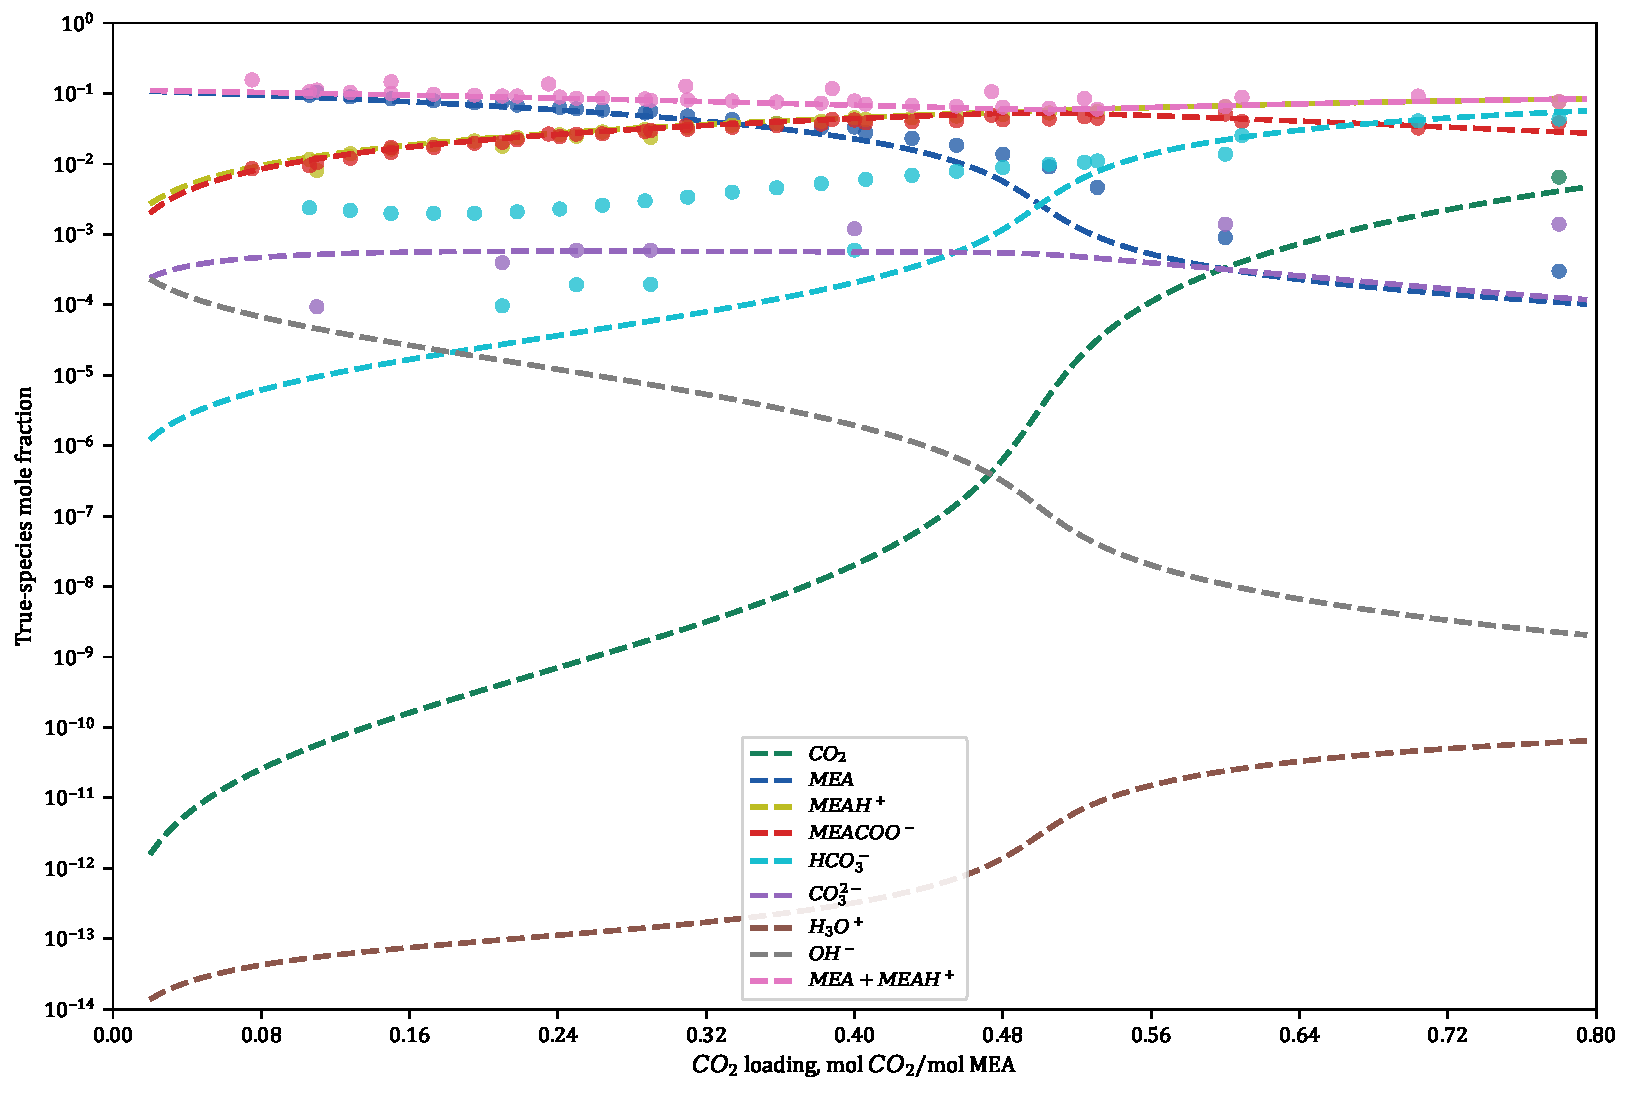
\includegraphics[width=\linewidth,height=0.27\textheight,keepaspectratio]{figures/mea_activity_speciation_20C.pdf}
        \par\smallskip
        \small (a) \SI{20}{\degreeCelsius}
    \end{minipage}
    \hfill
    \begin{minipage}{0.47\linewidth}
        \centering
        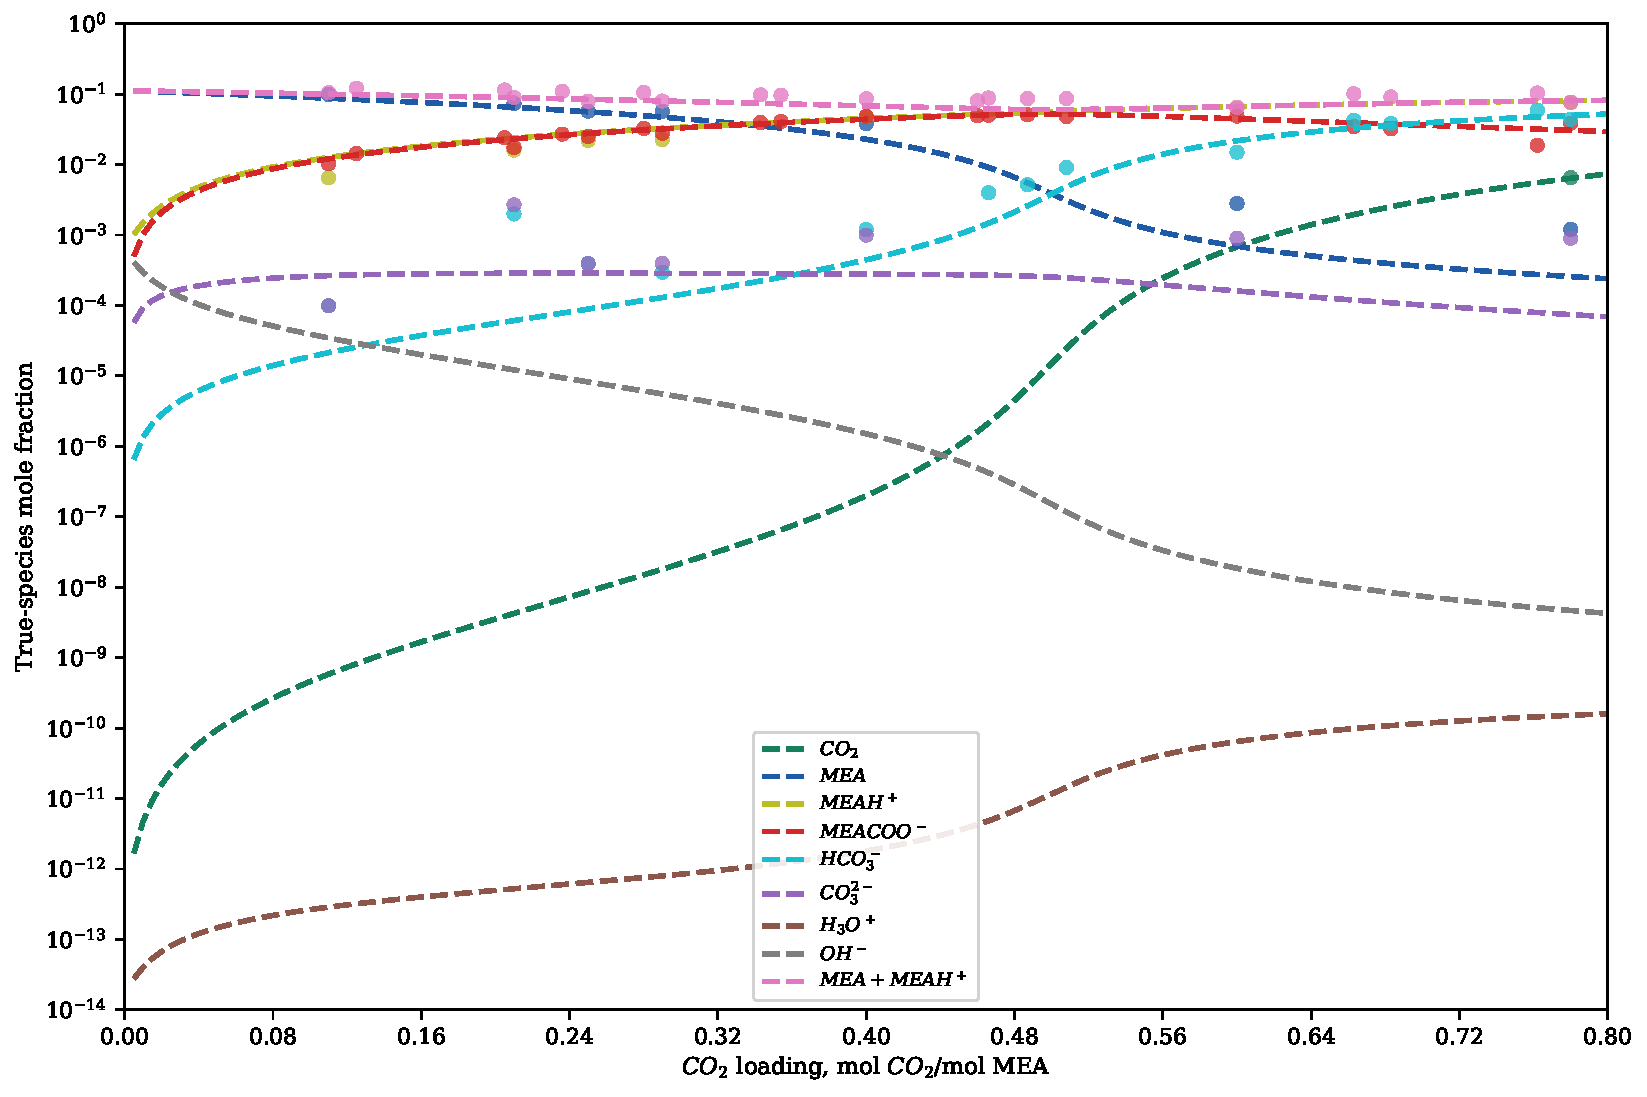
\includegraphics[width=\linewidth,height=0.27\textheight,keepaspectratio]{figures/mea_activity_speciation_40C.pdf}
        \par\smallskip
        \small (b) \SI{40}{\degreeCelsius}
    \end{minipage}
    \par\medskip
    \begin{minipage}{0.47\linewidth}
        \centering
        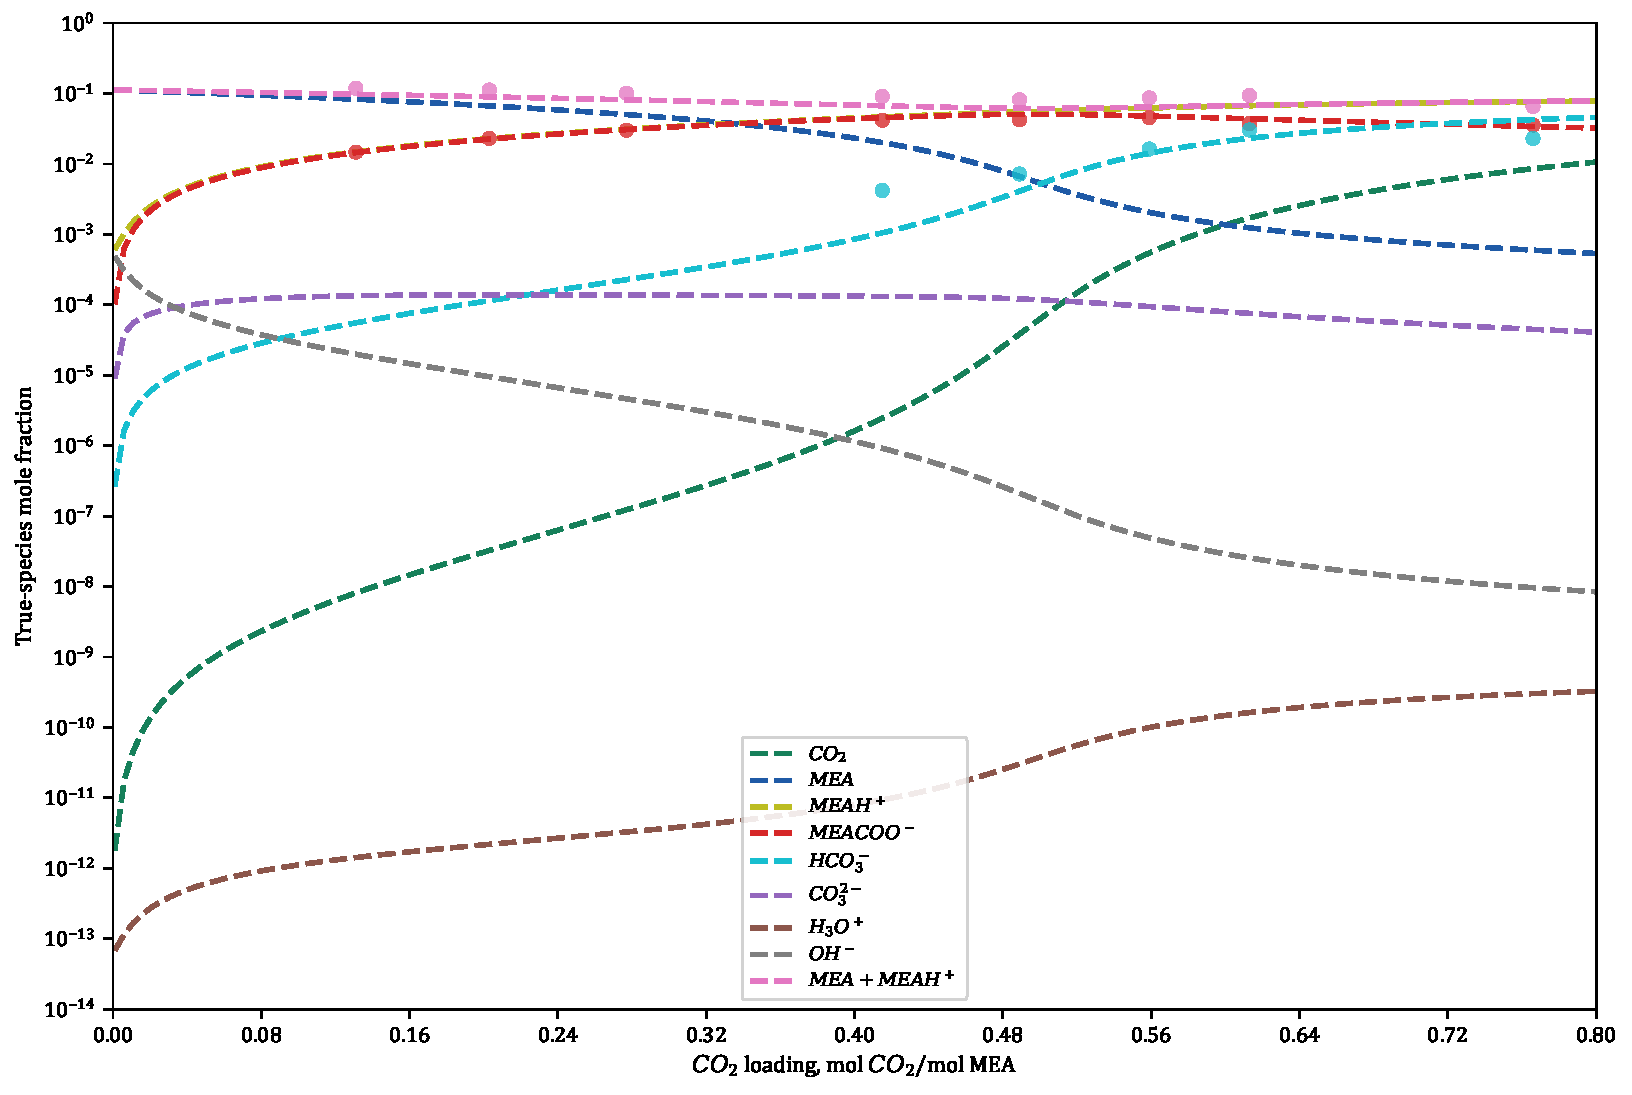
\includegraphics[width=\linewidth,height=0.27\textheight,keepaspectratio]{figures/mea_activity_speciation_60C.pdf}
        \par\smallskip
        \small (c) \SI{60}{\degreeCelsius}
    \end{minipage}
    \hfill
    \begin{minipage}{0.47\linewidth}
        \centering
        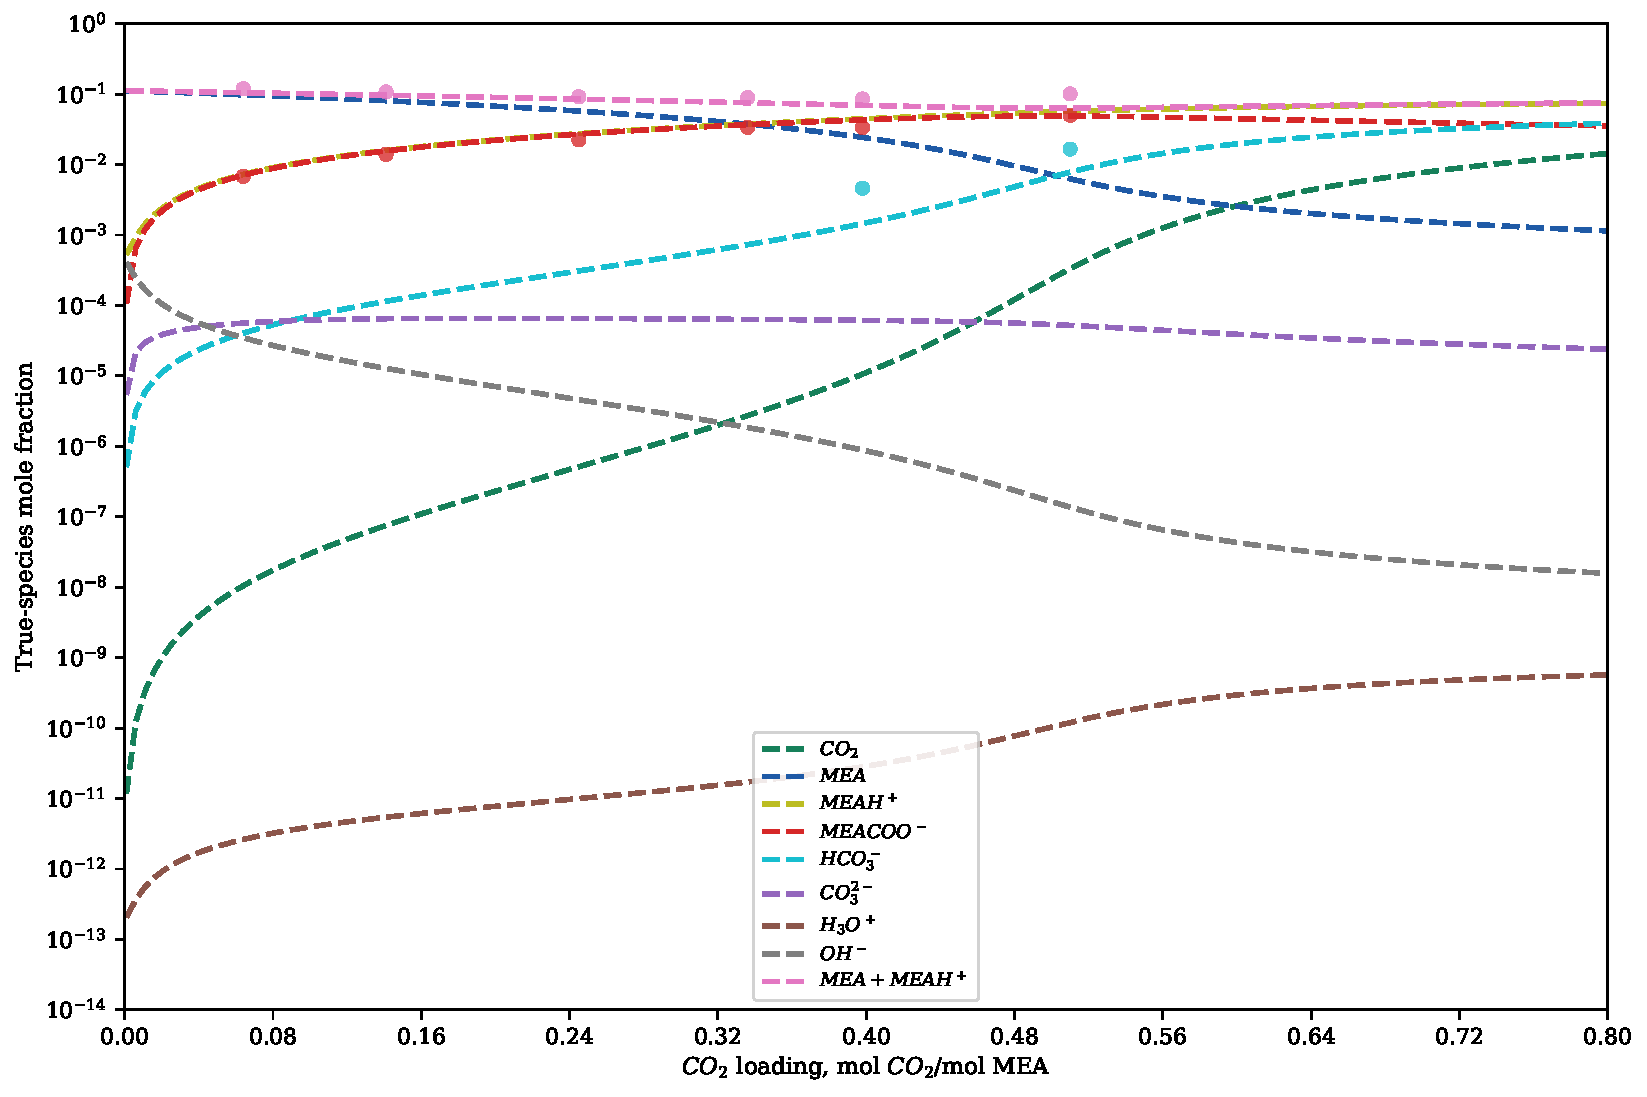
\includegraphics[width=\linewidth,height=0.27\textheight,keepaspectratio]{figures/mea_activity_speciation_80C.pdf}
        \par\smallskip
        \small (d) \SI{80}{\degreeCelsius}
    \end{minipage}
    \captionsetup{hypcap=false}
    \captionof{figure}{Activity-coupled ePC-SAFT speciation comparison for 30 wt\% \MEA.  Curves show the 642 accepted activity-coupled states, and markers show positive measured species or aggregate values.  Source-reported zero \HCOthree values enter upper-bound checks; balance-derived values are excluded from independent residuals.}
    \label{fig:activity-speciation}
    \end{minipage}
\end{center}

\subsection{CO2 solubility pressure response}
The controlled pressure comparison uses the same 31 Jou et al.\ measurements for both models.  The ideal baseline gives median absolute, signed median, and RMSE \(\log_{10}(P_{\mathrm{model}}/P_{\mathrm{data}})\) residuals of 0.160, \(-0.024\), and 0.297, respectively; the activity model gives 0.495, 0.226, and 0.565.  The activity model improves 4 paired records and worsens 27.  The ePC-SAFT parameterization therefore reduces pressure accuracy on this subset.

\begin{center}
    \begin{minipage}{\linewidth}
    \centering
    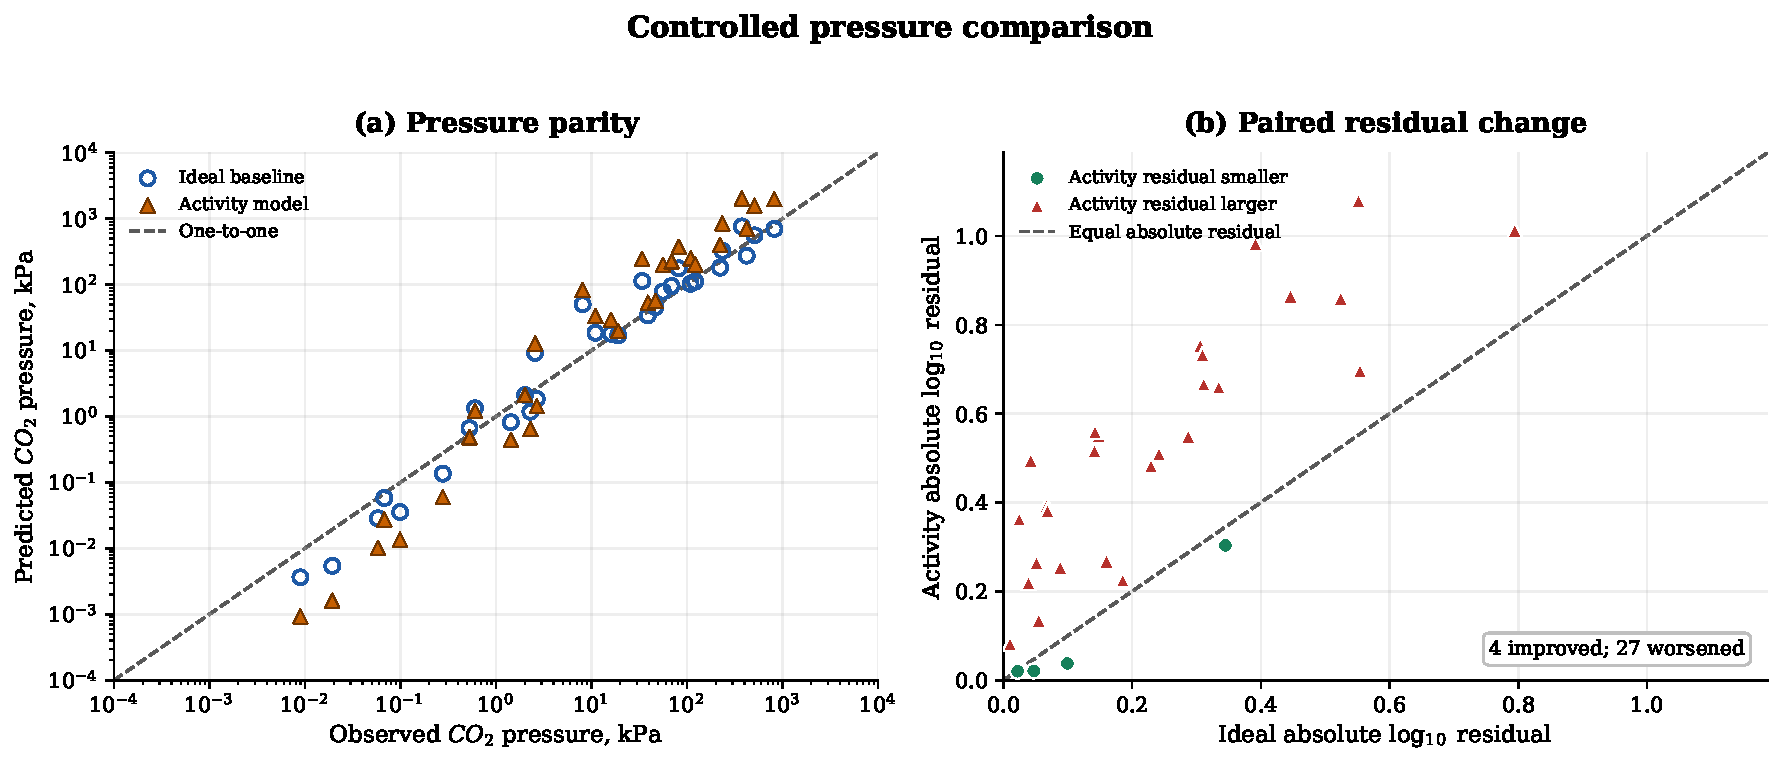
\includegraphics[width=0.96\linewidth,height=0.42\textheight,keepaspectratio]{figures/mea_controlled_pressure_comparison.pdf}
    \captionsetup{hypcap=false}
    \captionof{figure}{Controlled pressure evaluation using the same 31 Jou et al.\ measurements.  Panel (a) compares observed pressure with the ideal Smith--Missen baseline and activity-based ePC-SAFT calculation.  Panel (b) compares their absolute \(\log_{10}(P_{\mathrm{model}}/P_{\mathrm{data}})\) residuals; points below the one-to-one line favor the activity calculation.  The activity treatment reduces the absolute residual for 4 records and increases it for 27 records.}
    \label{fig:controlled-pressure-comparison}
    \end{minipage}
\end{center}

Across all 161 VLE records from six sources, the activity calculation gives median absolute, signed median, and RMSE pressure residuals of 0.493, \(-0.288\), and 0.645, respectively.  Because the ideal baseline was evaluated only on the 31-record Jou et al.\ subset, its metrics cannot be compared with this full-set summary.  The assembled pressure records contain no uncertainty values, so we report unweighted metrics.  Full-set pressure errors are largest between 40 and \SI{80}{\degreeCelsius} and decrease at \SI{120}{\degreeCelsius}.  The pressure residuals test gas--liquid equilibrium, while the NMR residuals test the liquid composition supporting that pressure.

\begin{center}
    \begin{minipage}{\linewidth}
    \centering
    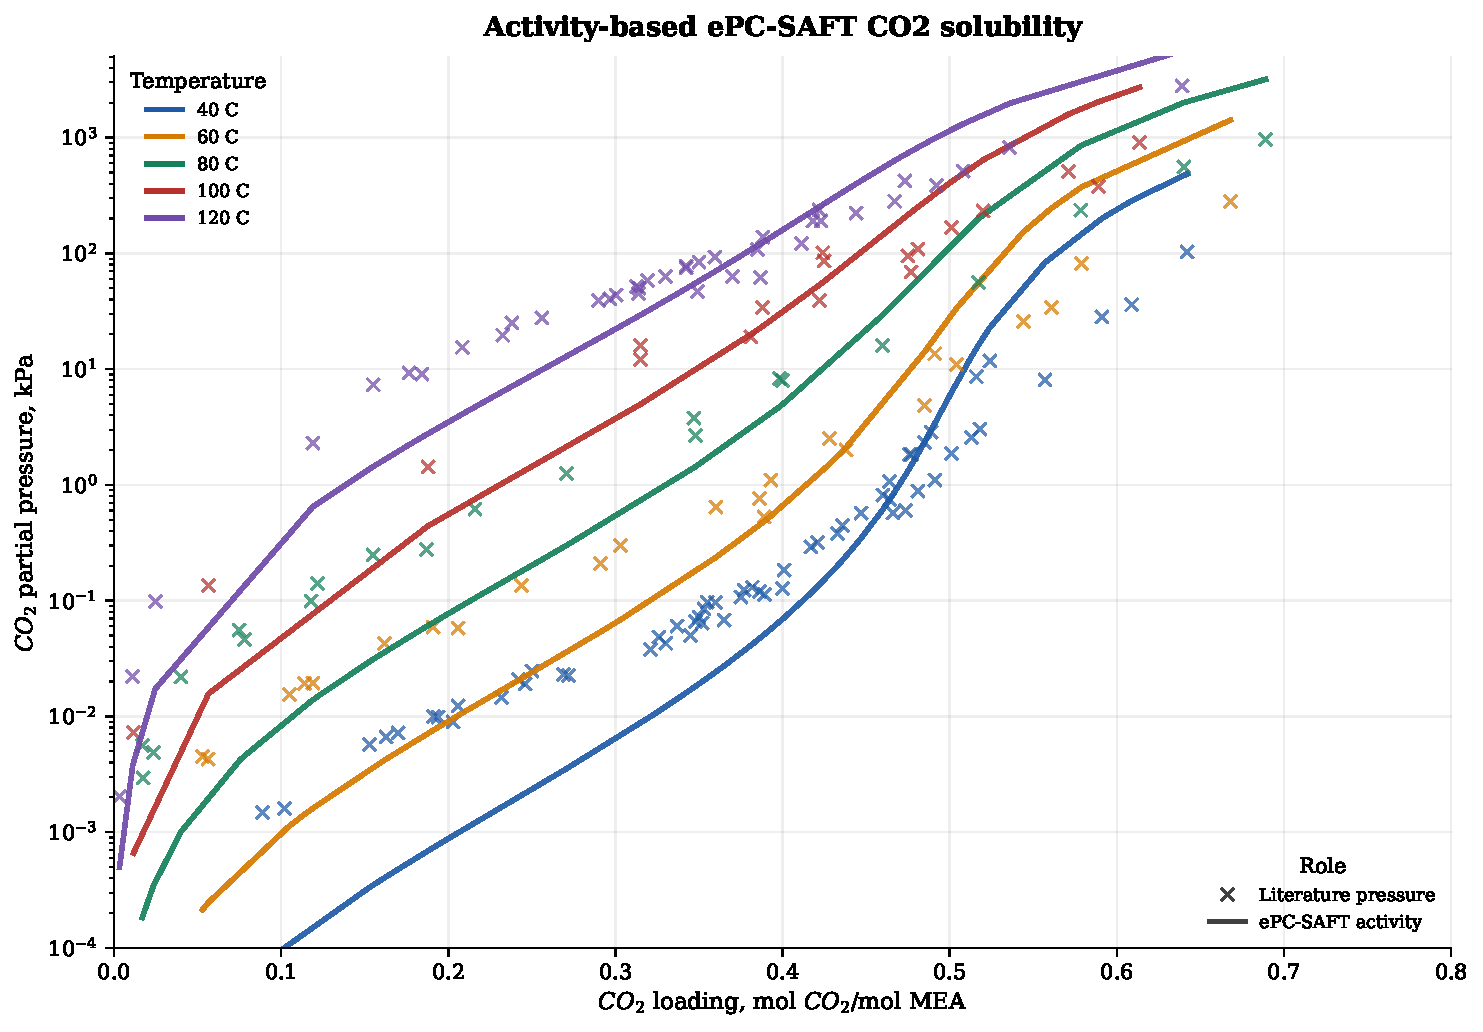
\includegraphics[width=0.84\linewidth,height=0.40\textheight,keepaspectratio]{figures/mea_activity_pressure_vs_loading.pdf}
    \captionsetup{hypcap=false}
    \captionof{figure}{Activity-coupled ePC-SAFT \COtwo-solubility pressure evaluation for 30 wt\% \MEA.  Connected curves show converged ePC-SAFT pressure rows at the assembled VLE loadings, and markers show the corresponding literature pressure records.}
    \label{fig:activity-pressure}
    \end{minipage}
\end{center}

\subsection{Sensitivity and identifiability}
The carbonate-family parameters are less identifiable than the amine-family parameters.  The NMR data include 53 positive \HCOthree and 16 positive \COthree observations, compared with 74 direct \MEACOO observations and 74 direct \ce{MEA + MEAH+} aggregate observations.  The reported calculation uses \(d_{\HCOthree}^{\mathrm{Born}}=3.0\) and \(d_{\COthree}^{\mathrm{Born}}=3.0\).  A carbonate-only sensitivity scan lowers the carbonate residual near \(d_{\HCOthree}^{\mathrm{Born}}=6.80\) and \(d_{\COthree}^{\mathrm{Born}}=3.00\).  We retain the 3.0/3.0 pair because the alternative is identified only by the carbonate observations used in the scan and lacks an independent pressure/speciation test.  \HthreeO and \Hydroxide are determined mainly by electroneutrality and water autoionization; the available NMR data provide no independent observations for either ion.

\begin{center}
    \begin{minipage}{\linewidth}
    \centering
    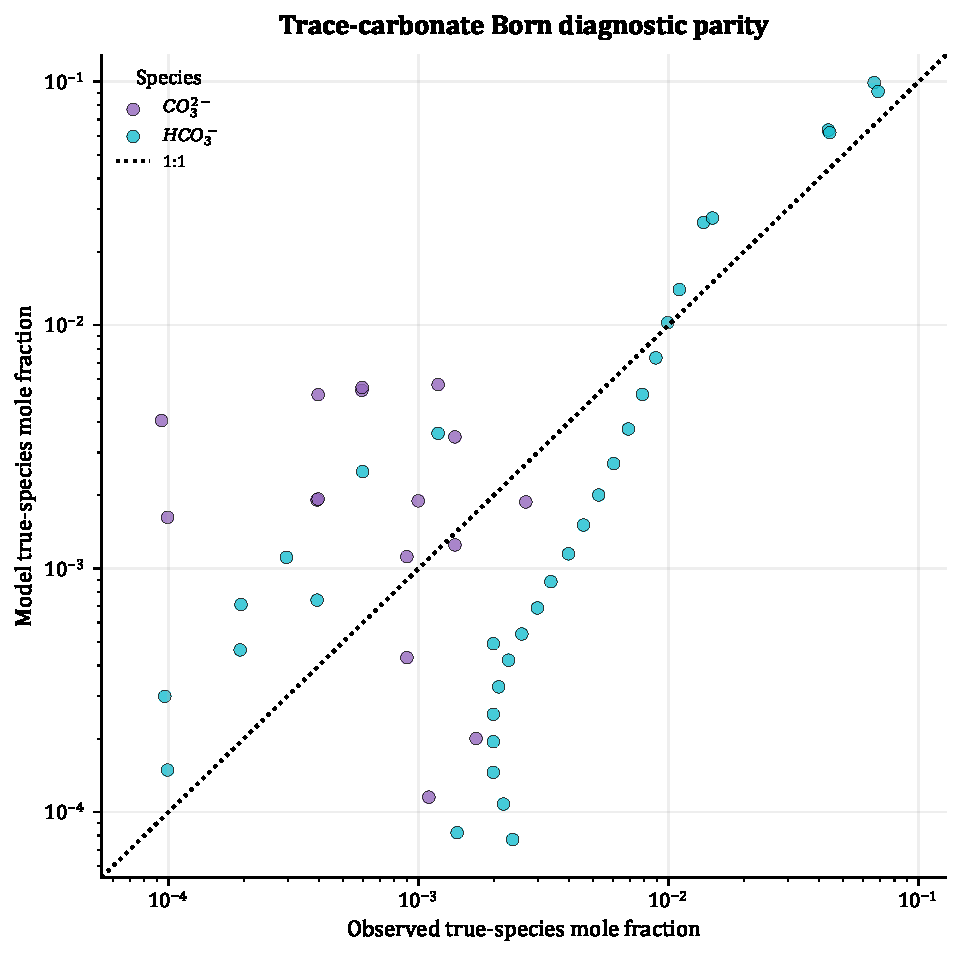
\includegraphics[width=0.64\linewidth,height=0.36\textheight,keepaspectratio]{figures/trace_carbonate_born_parity.pdf}
    \captionsetup{hypcap=false}
    \captionof{figure}{Carbonate-only Born-diameter sensitivity for \HCOthree and \COthree.  The reported calculation uses the 3.0/3.0 pair; the sensitivity scan shows that bicarbonate residuals vary strongly with the bicarbonate Born diameter.}
    \label{fig:trace-carbonate-born-regression}
    \end{minipage}
\end{center}

\subsection{Comparison with literature models}
\Cref{tab:literature-model-comparison} distinguishes apparent-chemistry PC-SAFT treatments, explicit-ion ePC-SAFT amine models, and advanced-Born electrolyte models for gas solubility.  The present calculation applies explicit-ion activity coupling and SSM+DS modified-Born solvation to carbamate-forming \MEA.  Following prior ePC-SAFT amine-solubility studies, the parameter estimation uses liquid-composition data while the VLE data test the predicted pressure~\cite{Uyan2015,Wangler2018}.

\subsection{Model limitations}
The seven fitted parameters reduce the squared NMR residual objective by 2.8\%, and the evaluation residuals remain much larger for bicarbonate and carbonate than for the amine family.  A local finite-difference screen is most sensitive to \(k_{\MEA,\HtwoO}\), \(k_{\COtwo,\MEA}\), and \(d_{\COthree}^{\mathrm{Born}}\); \(d_{\HthreeO}^{\mathrm{Born}}\) has little effect on the reported metrics.  The pressure comparison also shows that agreement with liquid speciation does not guarantee an accurate \COtwo pressure response.
